

\documentclass[12pt,oneside,final]{thesis}

\usepackage{mathtools}
\usepackage{setspace}
\usepackage{feynmp}
\usepackage{rotating}
\usepackage{cite}
\usepackage{amsmath,amsfonts}
\usepackage{amssymb}
\usepackage{graphicx}
%\usepackage{caption}
%\usepackage{subcaption}
\usepackage{mathrsfs}
\usepackage{color}
\graphicspath{{./figs/}}
\usepackage{fixltx2e}
\usepackage{array}

% wrapfig is fragile: use sparingly
\usepackage{wrapfig} 
%\usepackage{times}  % Use this for ugly fonts


\usepackage{fancyhdr}    % Use nice looking headers along with the required footer page numbers   
%\usepackage[hypertex]{hyperref}

\newcommand{\wpr}{\ensuremath{\mathrm{W}^\prime}}
\newcommand{\zpr}{\ensuremath{\mathrm{Z}^\prime}}
\newcommand{\bs}{\ensuremath{\mathrm{b}^{*}}}
\newcommand{\mum}{\ensuremath{\mathrm{\mu m}}}
\newcommand{\mus}{\ensuremath{\mathrm{\mu s}}}
\newcommand{\fbinv}{\ensuremath{\mathrm{fb^-1}}}
\newcommand{\pbinv}{\ensuremath{\mathrm{pb^-1}}}
\newcommand{\TeV}{\mathrm{TeV}}
\newcommand{\MeV}{\mathrm{MeV}}
\newcommand{\GeV}{\mathrm{GeV}}
\newcommand{\pt}{\ensuremath{\mathrm{p_{T}}}}
\newcommand{\MET}{\ensuremath{\mathrm{E_{T}^{miss}}}}
\newcommand{\textdegree}{\ensuremath{\mathrm{^{\circ}}}}

\makeatletter
\DeclareRobustCommand*\cal{\@fontswitch\relax\mathcal}
\makeatother

\DeclareGraphicsRule{.1}{mps}{*}{}
%Define the header/footer style
\pagestyle{fancy}
\fancyhf{}
\setlength{\headheight}{15pt}
\lhead{\leftmark}
\cfoot{\thepage}
\renewcommand{\headrulewidth}{0pt}
\fancypagestyle{plain}{% Redefine ``plain'' style for chapter boundaries
\fancyhf{} % clear all header and footer fields
\fancyfoot[C]{\thepage} % except the center
\renewcommand{\headrulewidth}{0pt}
\renewcommand{\footrulewidth}{0pt}}

%\tolerance=10000

%\makeglossary % enable the glossary

\begin{document}

\title{W prime stuff}
\author{Kevin Nash}
\degreemonth{September}
\degreeyear{2015} 
\dissertation
\doctorphilosophy
\copyrightnotice

% add your chaptders, best way is to have separate TeX files for each chapter
\chapter{Introduction}
\label{sec:intro}
\chaptermark{Theoretical Motivation}
Modern particle physics is described by a theory called the standard model (SM).  
The SM describes a universe in which matter consists of particles of half-integer spin\footnote{Intrinsic angular momentum} called fermions.  
These fermions interact with each other through force mediating integer spin particles called bosons.  
This section will provide a basic outline of this theory as well as the known issues and need for a more basic theory.

\section{Fundamental Particles}
The SM matter in the universe is around 98\% Hydrogen and Helium with the final 2\% being heavier elements.  
To a very good approximation, the known matter in the universe consists of protons, neutrons, and electrons.  
Electrons are categorized in the standard model as leptons and are fundamental.  
Protons and neutrons are composites of three quarks.  
The up quark (u) has +2/3e\footnote{e is the magnitude of the charge of the electron} charge, and the down quark (d) has -1/3e charge, so the proton is an up-up-down combination and the neutron is down-down-up.  
These quark compounds are called hadrons and are categorized into two families: baryons (three quarks), and mesons (two quarks).

Although this is a good approximation of the known universe, through experimental and theoretical advances we know that there are 
more exotic phenomena that can be described by extending the known quarks and leptons to three generations.  
The three lepton generations are defined by the electron, muon, tau and their corresponding neutrinos.
The +2/3e charge quarks are the up, charm, and top; whereas the -1/3e charge quarks are the down, strange, and bottom.  
These quarks and leptons are summarized in Table~\ref{table:SMferm} along with their charge and mass.
    
Quarks and leptons define all known fermionic matter, with bosonic particles being responsible for particle interactions.
    

\begin{table}[h]
\begin{center}
\begin{tabular}{l|c|c}
\hline
\hline
particle & charge (e) & mass (MeV)\\ \hline \hline
e & -1 & 0.5110 \\
$\mu$ & -1 & 105.7\\
$\tau$ & -1 & 1777\\
$\nu_{\mathrm{e}}$, $\nu_{\mu}$, $\nu_{\tau}$ & 0 & $<$ 2 $\times \mathrm{10^{-6}}$ \\
u & +2/3 & 2.3\\
d & -1/3 & 4.8\\
s & -1/3 & 95\\
c & +2/3 & 1.275 $\times \mathrm{10^3}$ \\
b & -1/3 & 4.18 $\times \mathrm{10^3}$\\
t & +2/3 & 173.2 $\times \mathrm{10^3}$\\
\hline
\end{tabular}
\end{center}
\caption{List of SM fermions with their charge and mass.  These particles all have spin 1/2.}
\label{table:SMferm}
\end{table}


\section{Fundamental Interactions}
Interactions in the SM can be described by the four fundamental forces: electromagnetic, weak nuclear, strong nuclear, and gravity.  
These forces manifest by the exchange of a corresponding elementary boson.  
The intrinsic properties of these force carrying particles are responsible for the range and relative strength of the interaction.


The electromagnetic force is responsible for well known phenomena such as molecular bonds.  
This force is mediated be the photon, a massless, charge-less, spin 1 particle.  
The photon interacts with charged particles only.        
The fact that the photon is massless leads to the infinite range of the electromagnetic force.  


The weak nuclear force manifests itself in nuclear decay, and is described by three force carrying bosons; the $\mathrm{W^+}$,$\mathrm{W^-}$, and Z.  
These bosons are massive, which leads to the weak force being short range.  
The $W^{\pm}$ bosons have integer charge whereas the Z boson is charge-less, and all three have spin 1.  
The weak force is responsible for transitions between flavors\footnote{The six quark types} of quarks (see Section~\ref{sec:weaktheory}).
Quarks and leptons alike interact by the weak force.


The strong nuclear force is responsible for binding quarks together to form hadrons.  
The strong force describes the interactions of particles that carry color.  
Color is an intrinsic property of fundamental particles, and has three varieties; red, green and blue.
This force is mediated by gluons, which are massless and interact with quarks.  
The strong force is the strongest and shortest range of the known forces.  
The theory behind the strong force is described in more detail in Section~\ref{sec:qcdtheory}

The known force carrying bosons and their properties are listed in table \ref{table:SMbos}

The fourth known force, gravity, is both the most recognizable and least understood of the forces.  
All attempts at including gravity into the SM have failed, but hypothetically gravity should be mediated by the spin 2 graviton, which interacts with massive particles..
Gravity is by far the weakest of the fundamental forces. 


\begin{table}
\begin{center}
\begin{tabular}{l|c|c|c}
\hline
\hline
particle & charge (e) & spin & mass (GeV)\\ \hline \hline
$\gamma$  & 0 & 1 & 0\\ 
$\mathrm{W^{\pm}}$ & $\pm$1 & 1 & 80.4\\
Z & 0 & 1 & 91.2\\ 
gl & 0 & 1 & 0 \\ 
gr & 0 & 2 & $<$ 6 $\times$ $\mathrm{10^{-38}}$ \\ 
\hline
\end{tabular}
\end{center}
\caption{List of SM force carrying bosons with their charge, mass and spin.  The graviton has not yet been observed.}
\label{table:SMbos}
\end{table}


\section{Feynman Diagrams}
Calculations in theoretical particle physics are facilitated by the use of feynman diagrams.  
Feynman diagrams are pictorial representations.  
These diagrams include the particles that interact (external lines), as well as the particles that mediate the interaction (internal lines), 
and where these external and internal lines intersect (vertices).
An example diagram is shown in Figure~\ref{figs:emuScattering}.  
The electrons interact with a photon ($\gamma$), and a force is observed.
This diagram represents electromagnetic repulsion (coulomb force).  

\begin{figure}
\begin{center}
\unitlength=1mm
\begin{fmffile}{feynman/emuScattering}
\begin{fmfgraph*}(40,30) \fmfpen{thick}
\fmfleft{i1,i2} \fmfright{sp1,sp2}
\fmf{fermion}{i1,v1,sp1}
\fmf{fermion}{sp2,v2,i2}
\fmf{photon,label=$\gamma$}{v1,v2}
\fmflabel{$e^-$}{i1}
\fmflabel{$e^+$}{i2}
\fmflabel{$e^-$}{sp1}
\fmflabel{$e^+$}{sp2}
\end{fmfgraph*}
\end{fmffile}
\end{center}
\caption{Feynman diagram depicting electron-positron scattering via
the electromagnetic interaction.}
\label{figs:emuScattering}
\end{figure}


The rules governing the calculation of physical observables from these diagrams are defined by the theory of Quantum Electrodynamics (QED).
Using these diagrams, the rules of QED let us calculate the matrix element ($\cal{M}$).  
$\cal{M}$ can by related to physical quantities through the square modulus ($|\cal{M}|^{\mathrm{2}}$), which is the probability density for a process to occur.   
From this, relevant quantities such as the cross section (see Section~\ref{sec:LumiXsec}) of the process can be calculated.  

Additionally, in the case that a particle decays we can evaluate the decay width ($\Gamma$).  
When a particle of mass M decays, there is a range of observed values of mass following a Breit-Wigner distribution centered at M.
The decay width represents the width of this distribution at half the maximum.  The average lifetime of the particle is 1/$\Gamma$.

For a given process there can be multiple contributing diagrams, for instance for a calculation involving the Coulomb attraction shown in Figure~\ref{figs:emuScattering}, 
one must also consider the 
diagrams shown in Figure~\ref{figs:emuScattering2}, which have the same incoming and outgoing particles.  
Diagrams such as this interfere with each other constructively or destructively in the calculation of the matrix element, 
which can increase or decrease the cross section of the full process.

\begin{figure}
\begin{center}
\unitlength=1mm
\begin{fmffile}{feynman/emuScattering1}
\begin{fmfgraph*}(40,30) \fmfpen{thick}
\fmfleft{i1,i2} 
\fmfright{sp1,sp2}
\fmf{fermion}{v1,i1}
\fmf{phantom}{v1,sp1}
\fmf{fermion,tension=0}{v2,sp1}

\fmf{phantom}{v2,sp2}
\fmf{fermion,tension=0}{sp2,v1}

\fmf{photon,label=$\gamma$}{v1,v2}

\fmf{fermion}{i2,v2}

\fmflabel{$e^-$}{i1}
\fmflabel{$e^+$}{i2}
\fmflabel{$e^+$}{sp1}
\fmflabel{$e^-$}{sp2}

\end{fmfgraph*}
\end{fmffile}
\end{center}
%\caption{Feynman diagram depicting electron-positron scattering via
%the electromagnetic interaction in the u channel.}
%\label{figs:emuScattering1}
\end{figure}


\begin{figure}
\begin{center}
\unitlength=1mm
\begin{fmffile}{feynman/emuScattering2}
\begin{fmfgraph*}(40,30) \fmfpen{thick}
\fmfleft{i1,i2} \fmfright{sp1,sp2}
\fmf{fermion}{i1,v1,i2}
\fmf{fermion}{sp2,v2,sp1}
\fmf{photon,label=$\gamma$}{v1,v2}

\fmflabel{$e^-$}{i1}
\fmflabel{$e^-$}{i2}
\fmflabel{$e^-$}{sp1}
\fmflabel{$e^-$}{sp2}


\end{fmfgraph*}
\end{fmffile}

\end{center}
\caption{Feynman diagram depicting electron-positron scattering via
the electromagnetic interaction in the u channel (top) and s channel (bottom).}
\label{figs:emuScattering2}
\end{figure}


Vertices in a Feynman diagram are points where energy and momentum are conserved in the calculation.  
Each of the vertices contributes a factor of the coupling constant $\alpha$ to the matrix element computation.  
In the calculation of the full matrix element for the electron positron attraction shown in Figures~\ref{figs:emuScattering} and~\ref{figs:emuScattering2}, 
we must consider diagrams with higher vertex multiplicity such as those seen in Figure~\ref{figs:emuScatteringnlo2}.  
To approximate $\cal{M}$ in QED, we can perform an expansion in the vertex multiplicity n, summing over matrix elements within the same order i ($\cal{M}_{\mathrm{i}}^{\mathrm{n}}$). 
 .  

\begin{figure}
\begin{center}
\unitlength=1mm
\begin{fmffile}{feynman/emuScatteringnlo1}
\begin{fmfgraph*}(40,30) \fmfpen{thick}
\fmfleft{i1,i2} \fmfright{sp1,sp2}
\fmf{fermion,tension=1.5}{i1,m1,v1,m2,i2}
\fmf{fermion}{sp2,v2,sp1}
\fmf{photon,label=$\gamma$}{v1,v2}
\fmf{photon,tension=0.0,left}{m1,m2}
\fmflabel{$e^-$}{i1}
\fmflabel{$e^-$}{i2}
\fmflabel{$e^-$}{sp1}
\fmflabel{$e^-$}{sp2}
\end{fmfgraph*}
\end{fmffile}
\end{center}
%\caption{Feynman diagram depicting NLO electron-positron scattering via
%the electromagnetic interaction.}
%\label{figs:emuScatteringnlo1}
\end{figure}

\begin{figure}
\begin{center}
\unitlength=1mm
\begin{fmffile}{feynman/emuScatteringnlo2}
\begin{fmfgraph*}(40,30) \fmfpen{thick}
\fmfleft{i1,i2} \fmfright{sp1,sp2}
\fmf{fermion}{i1,v1,i2}
\fmf{fermion}{sp2,v4,sp1}
\fmf{photon}{v1,v2}
\fmf{fermion,tension=0.5,left}{v2,v3,v2}
\fmf{photon}{v3,v4}
\fmflabel{$e^-$}{i1}
\fmflabel{$e^-$}{i2}
\fmflabel{$e^-$}{sp1}
\fmflabel{$e^-$}{sp2}
\end{fmfgraph*}
\end{fmffile}
\end{center}
\caption{Feynman diagram depicting NLO electron-positron scattering.}
\label{figs:emuScatteringnlo2}
\end{figure}


\begin{eqnarray}
\cal{M} = \sum\limits_{\mathrm{n=1}}^\infty \sum\limits_{\mathrm{i}}  \cal{M}_{\mathrm{i}}^{\mathrm{n}}
\label{eqn:matrixelement}
\end{eqnarray}  

Due to the fact that the coupling constant in QED is 1/137, this expansion can terminate quickly because high n diagrams contribute much less to $\cal{M}$.  
A calculation involving all diagrams with the least number of vertices is called leading order.  
Calculations involving all diagrams with higher order contributions as well are called next-to leading order (NLO), next-to-next-to leading order (NNLO), etc.    

Once the matrix element has been determined to an acceptable accuracy, we can extract the cross section in a straight forward manner.  
For the example electron-positron scattering process above the differential cross section has the following simplified equation due to the special case of identical mass particles:  

\begin{eqnarray}
\left(\frac{\mathrm{d\sigma}}{\mathrm{d\Omega}}\right)_{\mathrm{CM}} = \mathrm{\frac{|\cal{M}|^{\mathrm{2}}}{64 \pi^{2} E_{cm}^{2}}}
\label{eqn:xsecfromsigma}
\end{eqnarray}  


\section{Quantum Chromodynamics}
\label{sec:qcdtheory}
Quantum chromodynamics (QCD) is the theory describing the strong force, and is of particular importance for this thesis.  
The strong force is mediated by gluons which interact with particles that carry color.  
In QED, the photon is not charged, and thus can not interact with itself, however in QCD the gluon carries color and thus can interact with itself.  
Additionally, whereas the addition of a vertex greatly reduces the cross section in QED, the strong coupling constant $\alpha_s$ is of order 1, so 
higher order diagrams can contribute substantially to the measurement.  This means that QCD processes are much more difficult to calculate than QED 
processes.

However, $\alpha_s$ is not constant, and in fact increases as the distance scale of an interaction increases (see Figure~\ref{figs:alphasrunning}).  
This property of the the strong interaction is called asymptotic freedom.  For high $|q^2|$, $\alpha_s$ has the following form:

\begin{eqnarray}
\mathrm{\alpha_{s}(|q^2|)} =  \frac{\mathrm{\alpha_{s}(\mu^{2})}}{\mathrm{1+(\alpha_{s}(\mu^{2})/12\pi)(11n-2f)ln(|q^2|/\mu^{2})}}
\label{eqn:qcdalphas}
\end{eqnarray}  
%from Griffiths

where n is the number of colors (3), and f is the number of flavors (6), and $\mu^{2}$ is some arbitrary energy where $\alpha_{s}(\mu^{2})$ $<$ 1.
Therefore because 11n $>$ 2f, $\alpha_{s}$ will decrease as energy increases.


Therefore as the distance between two quarks increases, so do the forces holding them together.  
This large force at a characteristic distance ($\sim10^{-15}$ m) is the reason why it is difficult to observe a free quark (quark confinement).  
Although quarks can not be observed alone, there are ways of precisely determining the physical properties of free quarks through reconstruction of their decay products.  




\begin{figure}
\begin{center}
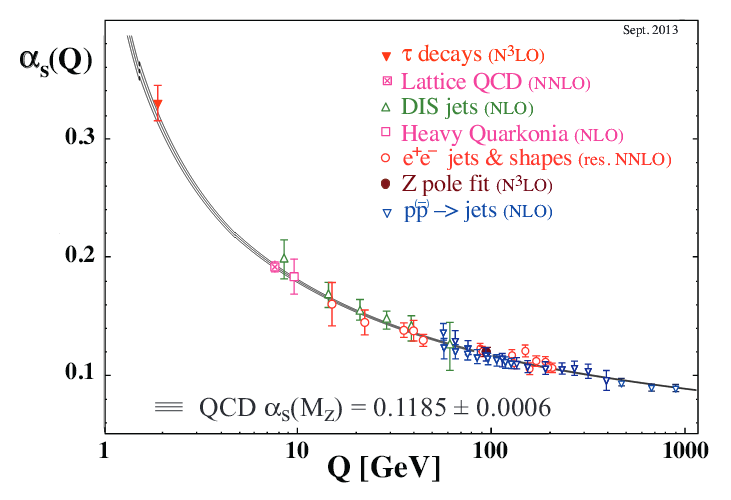
\includegraphics[width=1.0\linewidth]{figs/alphasrunning.png}
\caption{The QCD coupling constant $\alpha_{\mathrm{S}}$ as a function of the energy scale Q.}
\label{figs:alphasrunning}
\end{center}
\end{figure}
%from pdg


When a quark pair is produced with a high momentum, their separation increases quickly.  
As the separation of these quarks increases, the energy of the QCD field between them increases as well.  
If this separation is high enough, the energy between the quarks will reach a threshold where quark pair production is energetically favorable.  
At this threshold, the constituent quarks are then joined by these pair produced quarks.  
Additional quark pairs can be created many times, and the initial quark is detected as many hadrons that are collimated into a stream of particles called a jet.  
This process is called hadronization, 

The $\alpha_s$ parameter is low at short distances (or equivalently high energy); 
just like in QED, the impact of higher order diagrams is low.  
This allows the calculation of QCD diagrams using a finite perturbative expansion, and allows us to only consider only free quarks in high energy QCD calculations. 
The characteristic interaction energy where free quarks can be considered is around 400$\MeV$, which is much lower than energy scales 
considered in this thesis, so we will only be referring to free quark interactions.  


\section{The Weak Force}
\label{sec:weaktheory}
The weak force is felt by quarks and leptons alike.  
It is weaker than both the electromagnetic and the strong force, which leads to longer decay times for weakly decaying particles.  
The weak force is responsible for changing of quark flavor in an interaction.  
A vertex involving a change is quark flavor contributes a factor of $V_{ij}$ to the matrix element, where $V_{ij}$ is an element of the Cabibbo Kobayashi Maskawa (CKM) matrix 
(shown in Figure\ref{figs:CKM}).  
For example, the calculation of the diagram in Figure~\ref{figs:betaDecay} (beta decay) includes a factor of $V_{ud}$ = 0.97427.  
The CKM matrix is roughly diagonal, which means that a process which changes quark generation is rare.  

\begin{figure}
\begin{center}
\unitlength=1mm
\begin{fmffile}{feynman/betaDecay}
\begin{fmfgraph*}(40,30) \fmfpen{thick}
\fmfleft{i1,i2} \fmfright{sp1,sp2,sp3}
\fmf{phantom}{i2,v2,sp3}
\fmf{fermion}{i1,v1,sp1}
\fmf{fermion,tension=0.0}{v2,sp2}
\fmf{fermion,tension=0.0}{sp3,v2}
\fmf{photon,label=$W^{-}$}{v1,v2}
\fmflabel{$d$}{i1}
\fmflabel{$u$}{sp1}
\fmflabel{$e^-$}{sp2}
\fmflabel{$\nu_{e}$}{sp3}
\end{fmfgraph*}
\end{fmffile}
\end{center}
\caption{Feynman diagram depicting beta decay via
the weak interaction.}
\label{figs:betaDecay}
\end{figure}


Weak force interactions are dependent on the chirality of the interacting particle.
Chirality for massless particles is dependent on the relative orientation of the momentum and spin axes.  
Particles with momentum and spin aligned are referred to as right-handed, and particles with the momentum 
axis opposite to spin are left-handed\footnote{This convention is reversed for anti-particles}.
For massive particles this concept is generalized such that right- and left-handed components of a wavefunction 
can be extracted by using the right-handed operator (1+$\gamma^5$)/2 and the left-handed operator (1-$\gamma^5$)/2.  
The W boson only interacts with left-handed fermions whereas the Z boson interacts with right- and left-handed fermions with differing strengths. 

\begin{figure}
\begin{center}
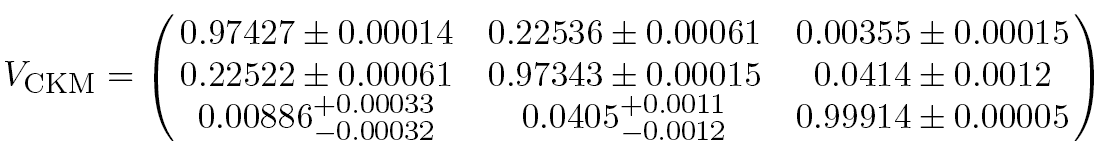
\includegraphics[width=1.0\linewidth]{figs/CKM.png}
\caption{The CKM quark mixing matrix.}
\label{figs:CKM}
\end{center}
\end{figure}



\section{Electroweak Symmetry Breaking}
%From pdg
Through the electroweak symmetry breaking mechanism, the mass of the W and Z bosons, and all fermions can be generated in the SM.  
We consider a scalar potenial of the form:
\begin{eqnarray}
\mathrm{ V(\Phi) = m^{2} \Phi^{\dagger} \Phi + \lambda ( \Phi^{\dagger} \Phi )^{2}  }\\
\mathrm{\Phi = \frac{1}{\sqrt{2}} \left( \frac{\sqrt{2} \phi^{+}}{\phi^{0} + ia^{0}}  \right)}
\end{eqnarray}  
where $\Phi$ is the Higgs field.  A plot of this potential can be seen in Figure~\ref{figs:higgspotential}.  
The minimum of the potential is not at V(0), and this point is unstable.  
The Higgs field has a non-zero vacuum expectation value (VEV).

\begin{figure}
\begin{center}
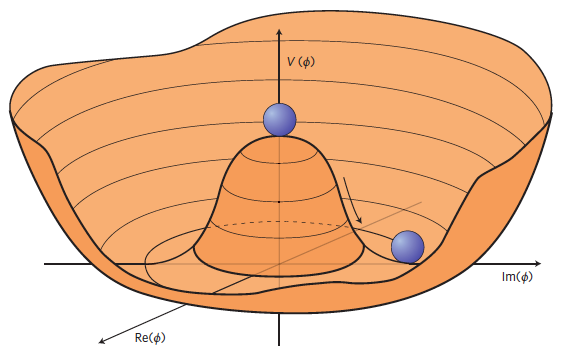
\includegraphics[width=0.7\linewidth]{figs/higgspotential.png}
\caption{The Higgs potential..}
\label{figs:higgspotential}
\end{center}
\end{figure}

Using the Higgs Lagrangian
\begin{eqnarray}
\mathrm{\cal(L) = (D_{\mu} \Phi )^{\dagger}(D_{\mu} \Phi ) -V( \Phi )}\\
(D_{\mu}\Phi) = (\partial_{\mu}+i g \sigma^{\alpha} W_{\mu}^{\alpha}/2 +i g^{'} Y B_{\mu}/2)\Phi
\end{eqnarray}  
we can extract the masses of the W and Z bosons as

\begin{eqnarray}
M_{W}^2 = \frac{g^{2}v^{2}}{4}\\
M_{Z}^2 = \frac{(g^{'2}+g^{2})v^{2}}{4}
\end{eqnarray}  

One new particle is predicted, a massive chargeless spin 0 particle called the Higgs boson.  
A particle consistent with the Higgs boson has been discovered in 2012 at the LHC.  
%https://cds.cern.ch/record/1638469/plots

  
\section{Beyond the Standard Model}
The SM is possibly the most successful theory in physics, but also one that is ultimately incomplete.  
We know that there are physical phenomena that the SM does not predict.  
The presence of dark matter and dark energy in the universe~\cite{Bennett:2003ba} is not currently explained by the SM.  
Given that dark matter and energy account for approximately 95\% of the universe, this is not a small issue.  
The SM does not explain the observation of neutrino oscillations~\cite{An:2012eh}, which implies that neutrinos have mass.  
The SM also does not naturally explain the relative values of fundamental constants such as why the weak force is $10^{33}$ times as strong as gravity.  
This issue is known as the hierarchy problem, and it is assumed that a complete theory would have a natural explanation for the seemingly random values of these constants.  

It is essential for a complete understanding of the universe that we probe beyond the standard model (BSM) theories that provide solutions to these issues.  
Theories involving compact extra dimensions~\cite{PhysRevD.64.035002} for example provide a natural explanation to the hierarchy problem.  
In these theories forces propegate in higher dimensions that are compactified.   
In this theory, the propagation of SM massive fields in higher dimensions leads to discrete modes, which are detectable as new massive particles.  
The propagation of the SM W or Z leads to excited modes that are referred to as the $\wpr$ and $\zpr$.
A novel way to look for BSM physics then is to attempt the creation and detection of massive states such as these bosons. 
In this thesis we discuss one such search for a W' boson.  

The W' boson is a particle predicted by many BSM theories such as Little Higgs~\cite{doi:10.1146/annurev.nucl.55.090704.151502}, 
Composite Higgs models~\cite{Vecchi:2013bja}, and Noncommuting Extended Technicolor~\cite{Chivukula:1995gu}.  





\chapter{Experimental Setup}
\label{sec:ExpSetup}
\chaptermark{Experimental Setup}
One way to search for BSM physics is to produce new particles directly.  
For this, we collide lighter particles at a high energy.  
The energy released in the collision can manifest in more massive particles\footnote{In SUSY there will usually be two} via mass-energy equivalence (E=m$\mathrm{c^2}$).
The collision may create one or more of these new particles, and from it's decay products an experimenter can reconstruct the properties of the new BSM massive state 
and study the properties (mass, decay width, spin, SM couplings etc.).  

For the measurements presented in this thesis, we collide high energy proton beams,  
which are designed to produce a high collision energy in comparison to fixed-target or electron-positron collisions.    
   
\section{Luminosity and Cross Section}
\label{sec:LumiXsec}
To understand how many occurrences of any physical process to expect in a set of collisions, we need to define at a minimum the concepts of luminosity, L, and cross section, $\sigma$.

The cross section of a process is a measure of the probability that a collision will produce the particles of interest.  
The phrase cross section refers to the physical cross section of a classical target and is thus measured in units of area.  
In a high energy collision, the cross section no longer refers to the physical dimensions of the target, and can be calculated directly from Feynman diagrams.  
The areas associated with these cross sections is very small and is measured in barns (b), which is $10^{-28} m^2$.  
BSM physics signatures have cross sections that are generally on the order of picobarns (pb) or femptobarns (fb).  
The process cross section is highly dependent of the energy of the collision and is why it is very important to have large, high energy accelerators for the discovery of new physics.  
The cross section of some SM processes are shown in Figure \ref{figs:SMxsecs}.


\begin{figure}
\begin{center}
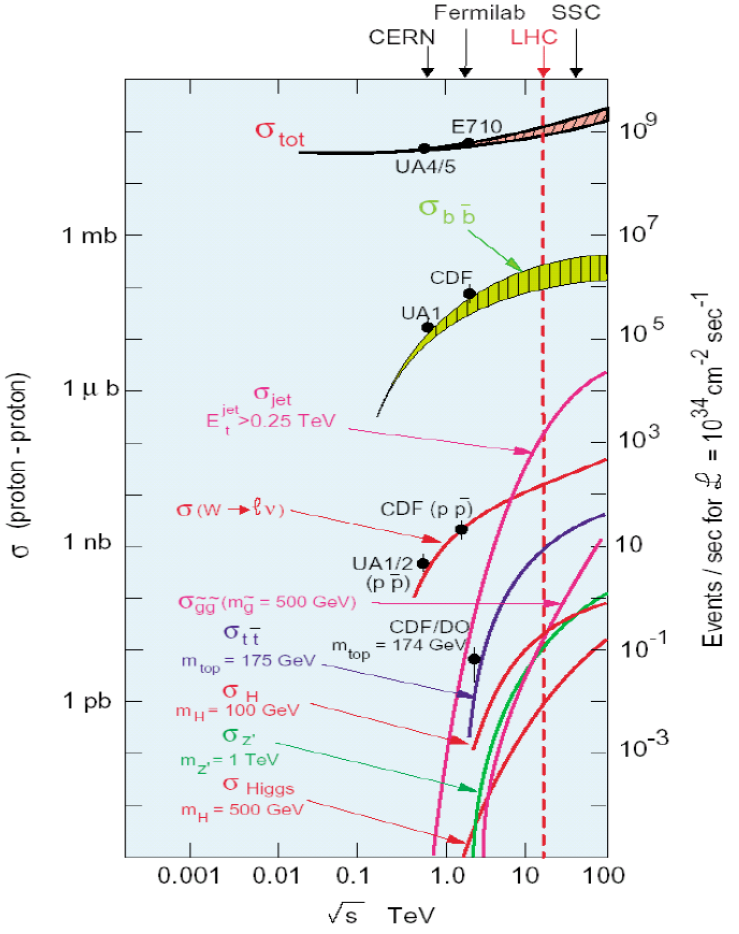
\includegraphics[width=0.7\linewidth]{figs/SMxsecs.png}
\caption{Standard model cross sections as a function of collision energy.}
\label{figs:SMxsecs}
\end{center}
\end{figure}


  
Luminosity is a measure of the intensity of the colliding beams and is the number of collisions expected per unit time per unit area.  
To look for BSM physics, we need to collect an ensemble of useful collisions (events), and thus higher luminosity leads to a larger 
ensemble, and consequently higher statistical precision of the measurement .  
Additionally, collecting data over time leads to a larger ensemble, so the time-integrated luminosity is a more useful variable to describe the total amount of data collected, 
which is reported in $\fbinv$.  Given in relevant collider properties, the luminosity can be defined as~\cite{Bayatian:922757}: 
\begin{eqnarray}
\mathrm{L = \frac{\gamma f k_{B} N_{p}^{2}}{4 \pi \epsilon \beta^{*}} F}
\end{eqnarray}  
where $\gamma$ is the Lorentz factor,  f is the frequency of revolution, $k_{B}$ is the number of bunches in the beam, $N_{p}$ is the number of protons per bunch, 
$\epsilon$ is the transverse emittance, $\beta^{*}$ is the betatron function, and F is a reduction factor based on the crossing angle.  

With these two concepts we can extract the predicted number of events, $N_{\mathrm{i}}$, for a given process i: 
\begin{eqnarray}
N_{\mathrm{i}} = \int L \mathrm{d}t \times \sigma_{\mathrm{i}} 
\label{eqn:Nevents}
\end{eqnarray}  

\section{The LHC}
The Large Hadron Collider (LHC) is a particle accelerator designed to reach collisions energies far surpassing any previous design.  
The LHC is a synchrotron that accelerates protons to 99.999997\% the speed of light.  
These protons beams are then collided at a center-of-mass energy ($\sqrt{s}$) of 8 $\TeV$.  
The accelerator segments and detectors at the LHC are shown in Figure~\ref{figs:lhc}.

% http://home.web.cern.ch/about/accelerators
% http://cds.cern.ch/record/1165534/files/CERN-Brochure-2009-003-Eng.pdf

A proton at the LHC starts out as hydrogen gas within the injector of LINAC 2 linear accelerator.  
The atoms are ionized using an electric field, stripping the electron.  
The resulting proton is accelerated using an oscillating electric field.  
The protons are accelerated in a straight line to an energy of 50~$\MeV$, or 31\% the speed of light.  

At this energy, linear acceleration is not practical, and the protons enter the Proton Synchrotron Booster (PSB).  The PSB is composed of four 157 m 
circumference superimposed synchrotrons that accelerate the protons using electric fields that are synchronized to the revolution frequency of the beams.  
The protons are kept on the circular accelerator with a magnetic field directed into the plane formed by the accelerator ring, which increases in strength as the protons gain energy.  
After the acceleration from the booster, the protons are at en energy of 1.4~$\GeV$, or 92\% the speed of light.

After the PSB, the protons enter the Proton Synchrotron (PS), a 628 m circumference synchrotron, which accelerates the protons to 25~$\GeV$, or 99.93\% the speed of light.  
After the PS, the protons enter the Super Proton Synchrotron (SPS), a 7 km circumference synchrotron, which accelerates the protons to 450~$\GeV$, or 99.9998\% the speed of light.

Finally, the beams enter the LHC.  This is the final synchrotron ring, with a circumference of 27 km.  
After the SPS, the protons are inserted into the LHC in one of two evacuated tunnels depending on which direction around the ring the beam is to travel.  

The LHC uses 1232 dipole magnets to keep the protons in the ring as they accelerate. which provide an 8.3 T field over their length.  
In order to deliver such a field, the magnets use superconducting niobium-titanium cables.  
These cables are cooled by superfluid helium to -271.3 C in order to achieve this superconductivity.  
During each revolution the energy of each proton in the LHC ring increases by 5 MeV.  
After being fully accelerated in the LHC, the protons are at an energy of 4~$\TeV$, or 99.999997 \%the speed of light.

The proton beams are then directed together for collisions in four positions around the ring.  
Each beam in the LHC ring contains 2808 bunches of protons, and each bunch contains 110 billion protons. 
These bunches need to be collimated in order to maximize collision frequency, which is accomplished by the use of 392 focusing quadrupole magnets.   
Each of these collision points houses its own detector, ALICE (A Large Ion Collider Experiment), ATLAS (A Toroidal LHC Apparatus), 
CMS (Compact Muon Solenoid), and LHCb (Large Hadron Collider beauty).  
The ALICE detector is primarily used for experiments involving heavy ion collisions that expand the current 
understanding of concepts such as the quark-gluon plasma and quark confinement   
LHCb is specialized for physics involving b quarks, such as measuring CP violation parameters from b-hadron interactions.  

CMS and ATLAS are large general purpose detectors.  
These detectors are used for many different types of physics searches, and are the two detectors responsible for the Higgs boson discovery.  
For the purposes of this thesis we will be concentrating on the CMS detector
  


\begin{figure}
\begin{center}
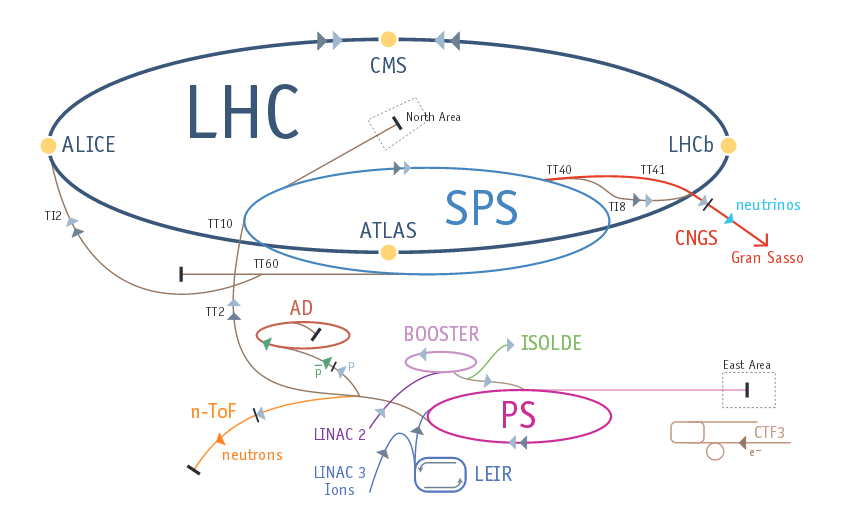
\includegraphics[width=1.0\linewidth]{figs/lhc.png}
\caption{A diagram of the LHC~\cite{lhcbrochure}.}
\label{figs:lhc}
\end{center}
\end{figure}
%http://cds.cern.ch/record/1092437/files/CERN-Brochure-2008-001-Eng.pdf

\section{CMS detector}
Here we will detail the basics of the CMS detector subsystems, for a more complete description, see Reference \cite{Bayatian:922757}.
The purpose of the CMS detector is to measure properties of particles that are created in a collision such as the energy and trajectory. 
The detector needs to collect enough information so that particles can be reconstructed and classified.  
Generally, we can reconstruct most physics signatures by analyzing electrons, muons, photon, charged hadrons, and neutral hadrons. 
The CMS detector has dedicated algorithms and systems that are specifically designed to identify each of these categories.  In order to reconstruct these particles, we impose a uniform axial magnetic field throughout the inner detector with the use of a superconducting magnet. 

The trajectory of charged particles is important for extracting information such as charge and momentum.  
The process of reconstructing the trajectory of these  particles is called tracking.  
Near the interaction point tracks are very dense, and tracking becomes very difficult.  
In this region we use a fine array of silicon pixels that register a charge particles position based on charge deposited in the device.  
Additional measurements are made by a second series of silicon detectors called the Silicon Strip Tracker. 
Using a series of these position measurements, we can fit a charged particle track.  

Energy can be measured by the use of calorimeter systems.  
A calorimeter is a detector designed such that a particle will deposit all of its energy within its volume in the form of photons, 
which can be detected to extract a measure of the total energy. 
These systems are subdivided into the Electromagnetic Calorimeter (ECAL) and Hadronic Calorimeter (HCAL).  
The ECAL uses scintillation crystals to detect particles that interact primarily with the electromagnetic force such as electrons and photons.  
Hadrons pass through the ECAL with minimal loss and deposit energy in the HCAL, which uses layers of absorber and scintillator to first 
create a shower of secondary particles, and then measure the total energy of these secondary particles.  

The detection of muons requires a specially designed system that lies outside of the ECAL, HCAL, and magnet.  
Muons pass through the ECAL and HCAL without losing a substantial fraction of their energy.  
To reconstruct the trajectory of muons, we use several different systems both inside and outside the magnet.

See Figure~\ref{figs:CMSdiagram1} for a diagram of the full detector, and Figure~\ref{figs:CMSdiagram} for a cross-sectional view of the detector subsystems.

\begin{figure}
\begin{center}
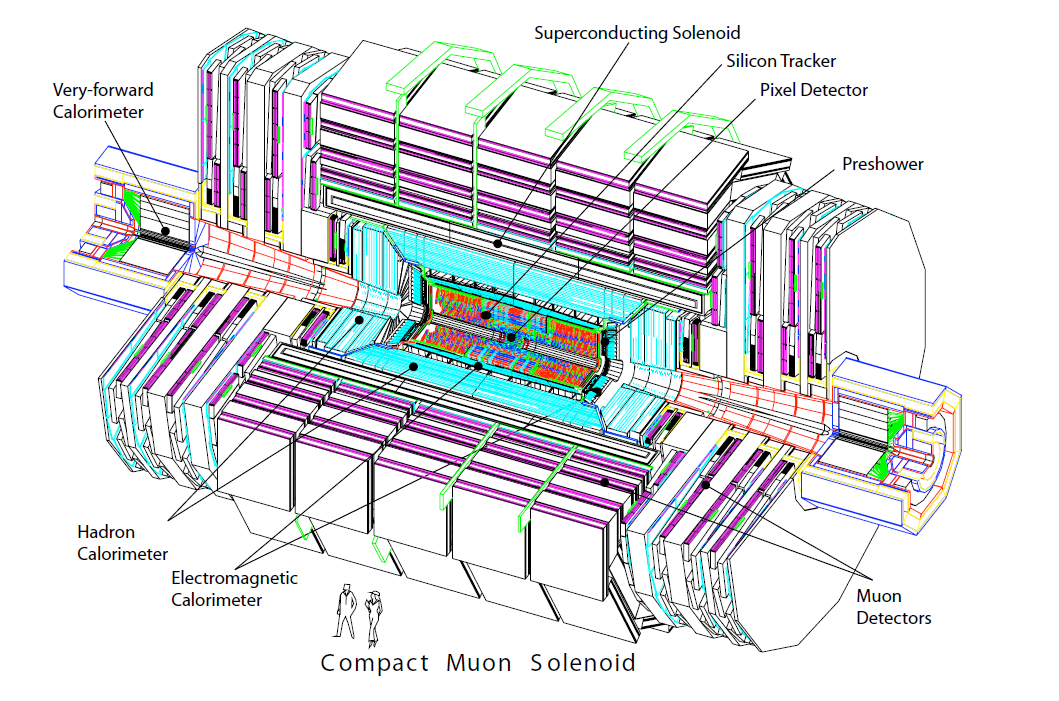
\includegraphics[width=1.0\linewidth]{figs/CMSdiagram1.png}
\caption{A diagram of the full CMS detector.}
\label{figs:CMSdiagram1}
\end{center}
\end{figure}

\begin{figure}
\begin{center}
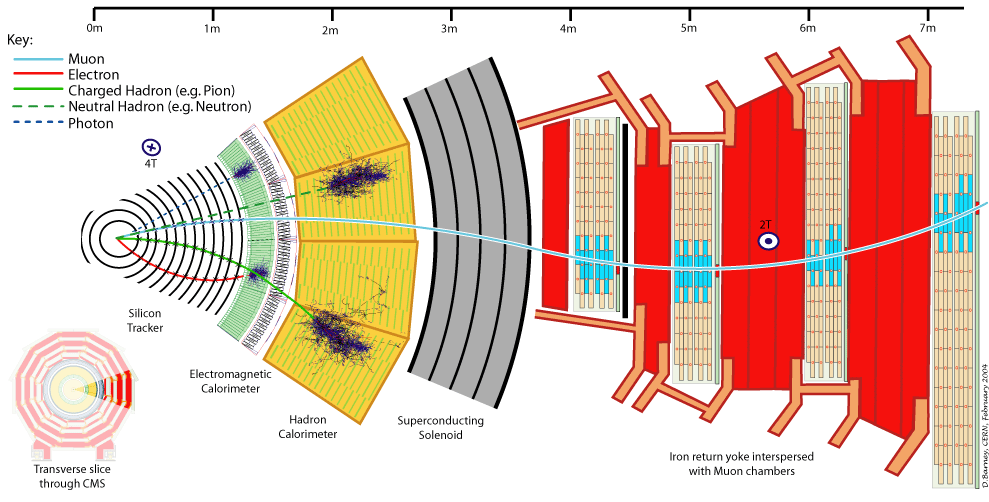
\includegraphics[width=1.0\linewidth]{figs/CMSdiagram.png}
\caption{A cross-sectional view of the CMS detector.}
\label{figs:CMSdiagram}
\end{center}
\end{figure}



\subsection{Pixel Tracker}
The closest detector system to the interaction point is the silicon pixel tracking system (see Figure \ref{figs:CMSpixel}).   .  
This system extends from a radius of 4 cm to 11 cm in the barrel, and is designed to track charged particles in a very dense environment.  
This is achieved with three arrays of two dimensional silicon pixels placed at a radii of 4.4 cm, 7.3 cm, and 10.2 cm, as well as two endcap disks for a total of 65 million pixels.  
When a charged particle traverses one of the 100 $\mum$ $\times$ 150 $\mum$ pixels, it imparts enough energy to the silicon to eject an electron.  
The electrons and their corresponding hole are detected on the pixel surface as a signal.  
This signal allows us to extract a position measurement for the charged particle.  

The entire system exists in a magnetic field, so the trajectory of the electrons and holes are deflected in the r,$\phi$ plane before detection.  
The angle of this Lorentz drift is 23$\textdegrees$, which causes the electron-hole pairs to be detected over a wide region covering multiple pixels.  
This effect improves the spacial resolution to 10 $\mum$ in r-$\phi$ space due to the fact that the charge center can be reconstructed by more measurements, 
whereas the z resolution is 20 $\mum$ due to the fact that there is no magnetic deflection in this direction. 
The pixel detectors in the endcap disks are angled at 20$\textdegrees$ in a turbine-like design to take advantage of this effect.  

  

\begin{figure}
\begin{center}
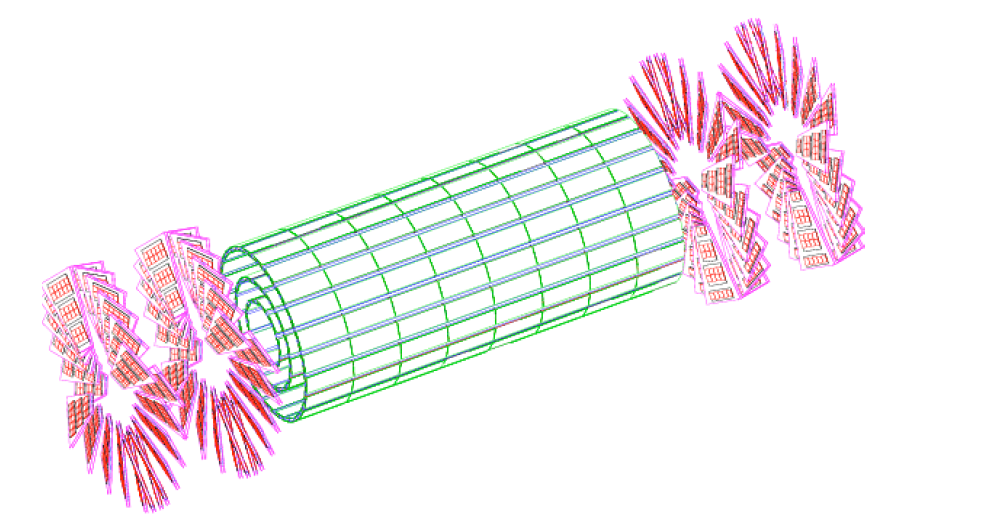
\includegraphics[width=1.0\linewidth]{figs/CMSpixel.png}
\caption{A diagram of the pixel detector.}
\label{figs:CMSpixel}
\end{center}
\end{figure}
  
\subsection{Silicon Strip Tracker}
Outside of the silicon pixel tracker (see Figure \ref{figs:CMStracker}) out to a radius of 130 cm in the barrel lies the silicon strip tracking system.  

The system in segmented into the inner barrel, outer barrel, inner disk, and endcap segments.  
The inner barrel segment (20 cm $<$ r $<$ 55 cm) uses four arrays of 10 cm $\times$ 80 $\mum$ silicon microstrips .  
The outer barrel (55 cm  $<$ r $<$ 130 cm) uses six arrays of large pitch 25 cm $\times$ 180 $\mum$ silicon microstrips.  

The endcap silicon strip detector consists of nine disks from 120 cm  $<$ z $<$ 280 cm.  
The inner disk segment contains three smaller disks that connect the inner barrel and endcap segments.  

\begin{figure}
\begin{center}
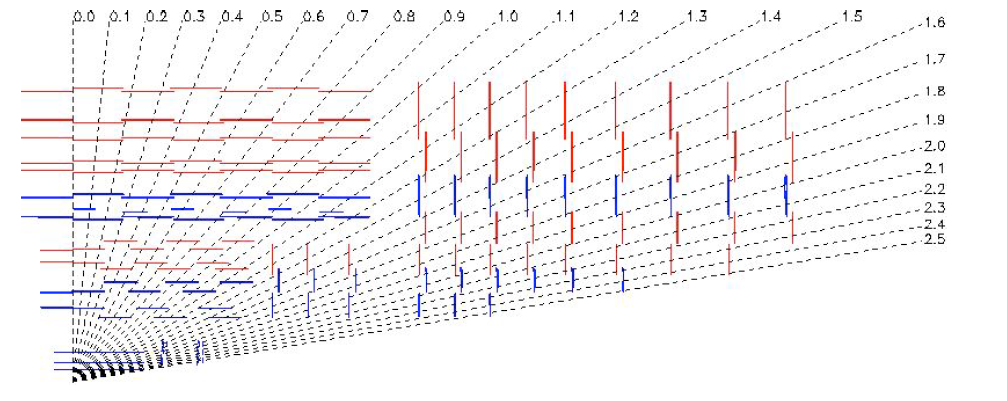
\includegraphics[width=1.0\linewidth]{figs/CMStracker.png}
\caption{A diagram of the silicon tracking system.}
\label{figs:CMStracker}
\end{center}
\end{figure}
  


%\subsection{Preshower Calorimeter}
\subsection{Electromagnetic Calorimeter}
The ECAL (see Figure~\ref{figs:CMSecal}) is designed to provide energy information for electrons and photons.  
These particles will typically deposit all of their energy within the detector, which is detectable as photons. 

To do this, the ECAL uses 61200 lead tungstate ($\mathrm{PbWO_4}$) scintillation crystals in the barrel and 7324 in each endcap.  
Lead tungstate is chosen as a scintillation material because it has a short radiation length (0.89 cm), fast response (25 ns for 80\% of light), and can 
withstand harsh radiation environments (10 Mrad).
The light emitted is around 30 photons per $\MeV$ for the energy of the particle of interest, which is somewhat low.  
Therefore, the ECAL uses avalanche photodiodes in the barrel and voltage phototriodes in the endcap segments to amplify the signal upon readout.  

The endcap regions of the ECAL include a preshower detector that is used to distinguish high energy photons from decaying pions.  
A pion decaying to two closely spaced photons can mimic one high energy photon to the 2.2 cm wide ECAL crystals.  
The preshower is able to distinguish these events with a finer granularity (2 mm) silicon strip detector.   
 
\begin{figure}
\begin{center}
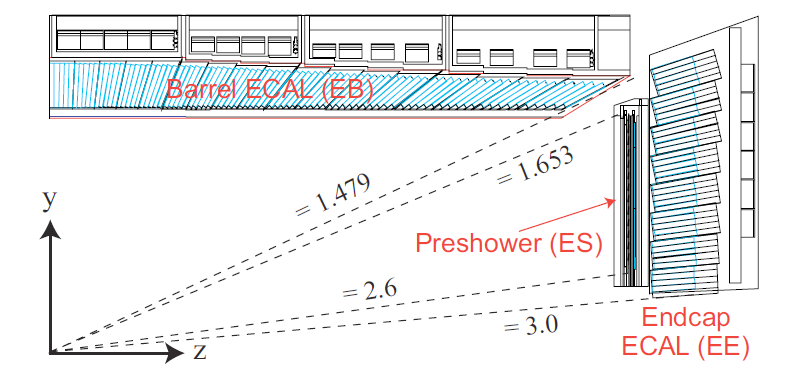
\includegraphics[width=1.0\linewidth]{figs/CMSecal.png}
\caption{A diagram of the ECAL system.}
\label{figs:CMSecal}
\end{center}
\end{figure}
  





\subsection{Hadronic Calorimeter}
The HCAL (see Figure~\ref{figs:CMShcal}) is designed to give the energy of charged and neutral hadrons, which generally lose very little energy in the ECAL.  
The HCAL is segmented into the inner barrel (inside the magnet), outer barrel (outside the magnet), endcap, and forward (close to the beamline).  

The HCAL uses alternating layers of absorber and scintillator to calculate the energy of these hadrons.  
The absorber creates a cascade of secondary particles that emit photons in the scintillator which can then be detected and summed to reconstruct the energy of the initial hadron.  
The photons emitted in the scintillator are carried to the photodetectors by optical waveguides.  
The HCAL uses hybrid photodiodes to detect the scintillation light and provide a signal that can be used to extract the total energy of the hadron.  

\begin{figure}
\begin{center}
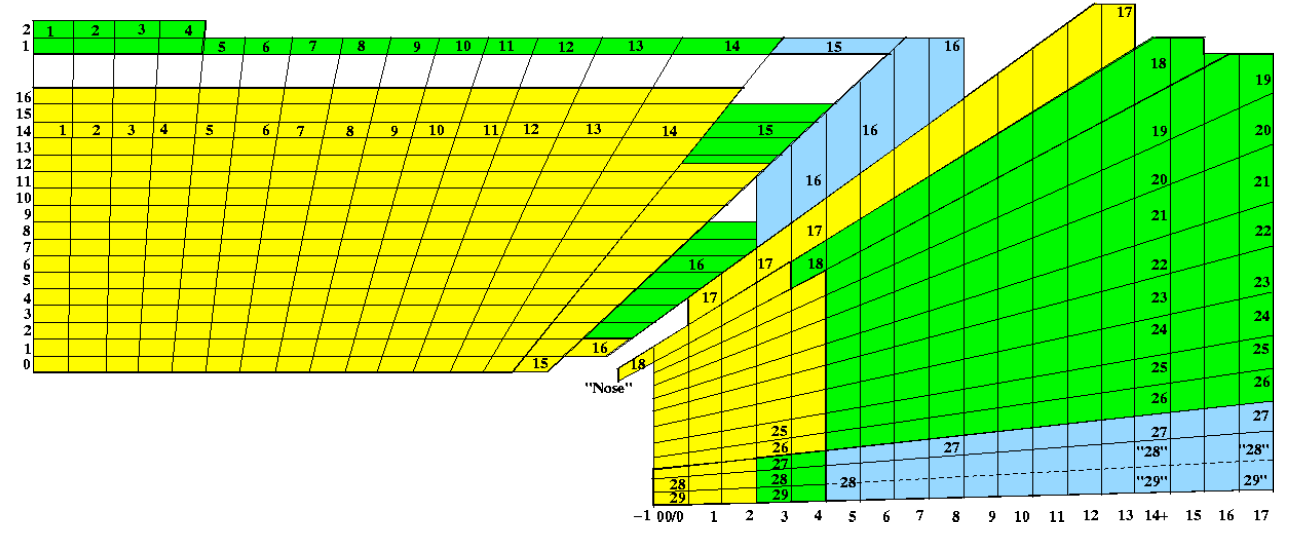
\includegraphics[width=1.0\linewidth]{figs/CMShcal.png}
\caption{A diagram of the HCAL system.}
\label{figs:CMShcal}
\end{center}
\end{figure}
  
\subsection{Magnet}
A charged particle moving perpendicular to a magnetic field follows a helical trajectory.  
The curvature of this helix is dependent on the momentum of the particle, and the handedness is dependent on the charge.  
Therefore, by immersing the tracking volume in an axial magnetic field we can get an accurate measurement of these properties.  
The stronger the magnetic field, the more precise these measurements can be for a high energy particle due to the more distinct curvature.  
To produce this field, CMS employs the largest superconducting magnet ever built.  

The design goal for the magnet is to be able to reproduce high momentum muons.  
The benchmark used for this is to have a momentum resolution of $\Delta$p/p $\leq$ 10\% at a muon momentum of 1 $\TeV$.  
To achieve this, we employ a solenoid with a length of 12.9 m and bore of 5.9 m.  
The coils of this solenoid are superconducting niobium-titanium, which produce a uniform 3.8 T magnetic field in the interior. 
The coils are wound in four layers, for a total of 2168 turns that carry 19.5 kA of current.    

The magnet additionally provides structural support to withstand the weight of the CMS detector as well as the magnetic force exerted from it's own magnetic field.  

\subsection{Muon System}
The reconstruction of muons and electrons starts at the inner silicon tracking system.  
Whereas electrons deposit their energy in the ECAL, a muon will traverse the ECAL and HCAL without significant interaction because a muon is around 200 times as massive.  
Muons are of interest to the Higgs discovery as well as BSM physics, 
and an accurate determination of the muon energy is also required for determination of the total event energy and missing energy.  
Therefore, the CMS detector has a large system purely designed to reconstruct muons, which lies outside all other detector systems at CMS.  

The muon system is comprised of a gaseous detectors interleaved with iron.  
The iron is saturated with the return field of the magnet, which creates a magnetic field at one half of the internal field strength and oriented in the opposite direction.  
The three layers of this ``return yoke" system bends muons to get an accurate measure of the momentum outside of the magnet.  

The trajectory of the muons is reconstructed with three types of gaseous detectors.  
The detectors work on the same basic principle, where an incoming muon ionizes the gas creating an electron-hole pair.  
The electron is detected by the anode, and the hole is detected by a cathode.  
A coincidence of these two measurements gives a measure of the position and time that a muon traversed the detector.  
With a series of these measurements, a trajectory can be fit, and physical quantities of interest can be reconstructed.  

In the barrel region ($|\eta|$ $<$ 1.2), drift tubes are used because the neutron flux and magnetic field are low.  
A drift tube is a detector consisting of a gas filled tube with an anode wire.  
The ionized electron from the gas volume travels to the anode wire, and a measurement of position is made.  
The detection of this electron registers the position along the wire (z coordinate).  
The r-$\phi$ coordinate within the drift tube cross sectional can be calculated by using the drift time of the ionized electrons to the anode.  

In the endcap region, where the magnetic field and neutron flux are high, cathode strip chambers are used.  
Cathode strip chambers are trapezoidal in shape with six gas gaps for ionization.  
These gas gaps each have one plane of cathode strips pointing radially outward and one plane of anode wires oriented perpendicular to the cathode.  

In both the barrel and endcap regions, resistive plate chambers are used.  
These detectors are composed of two parallel resistive plates separated by a gas gap.  
The design goal of the resistive plate chambers is to complement the cathode strip chambers and drift tubes to give two independent measurements of position.  
Additionally, resistive plate chambers offer very quick and accurate time resolution.  This offers a 
quick approximation of the muon momentum which is useful for the trigger system and matching a muon track to a bunch crossing.  

The muon system and inner tracker both contribute to the trajectory measurement of a muon.  
In terms of momentum resolution, the inner tracker offers much better sensitivity up to around 200 $\GeV$.  
After 200 $\GeV$, the muon system starts to significantly improve the momentum measurement.

Figure \ref{figs:CMSmuon} shows a diagram of the muon system.  
\begin{figure}
\begin{center}
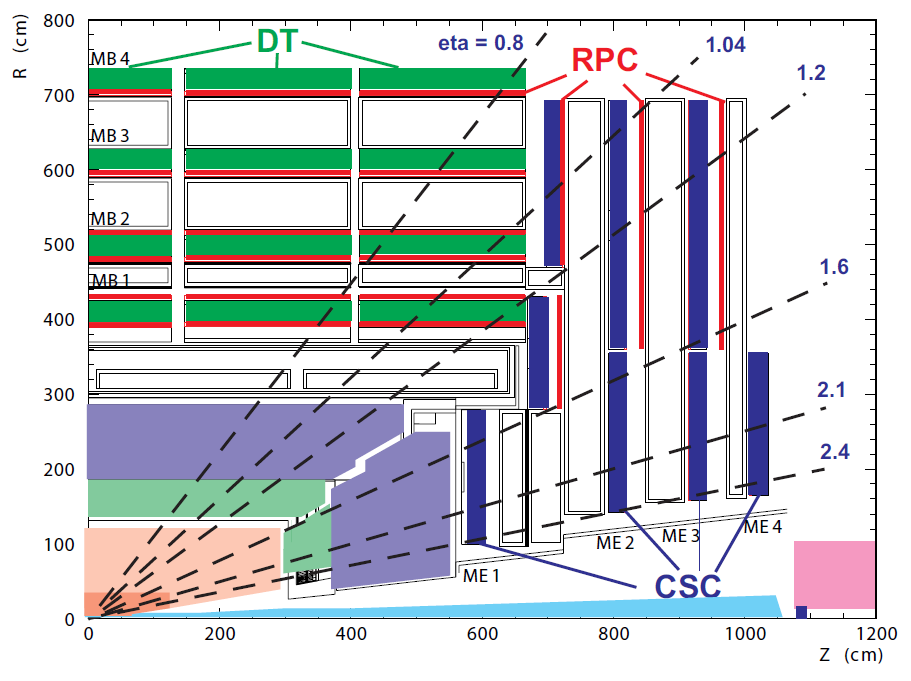
\includegraphics[width=1.0\linewidth]{figs/CMSmuon.png}
\caption{A diagram of the muon system.}
\label{figs:CMSmuon}
\end{center}
\end{figure}

\subsection{Trigger}
The LHC delivers around 1 billion proton-proton collisions per second.  
However, because of the current computing limitations, the CMS detector system can only write around 100 collisions per second as data.  
Therefore, a trigger system is developed to distinguish the most potentially interesting physics signatures.  

The L1 trigger takes information from the calorimeter and muon systems and their correlations.  
When one of these detectors produces a signal, the information takes 3.2 $\mus$ to reach the L1 processing area and return to the detector.  
The L1 processing time for the information for a maximum of 1 $\mus$ where the decision is made to keep the event to search for potential physics signatures.  
The L1 has various algorithms designed to keep ``trigger primitives", which can be objects such as high $\pt$ muons, electrons, jets or full event information like total energy or $\MET$.  
The L1 trigger only saves on average of 1 out of every 1000 events.  

After the L1 trigger, the trigger primitive events are processed by the high level trigger (HLT).  
The HLT again saves only 1 out of 1000 of these events.  
The processing time for the HLT algorithm is longer than the L1 system, and to extract the potentially exciting physics objects the algorithm performs partial event reconstruction.  
An event that enters the HLT algorithm is first analyzed based on the output of the calorimeters and muon system, then pixel tracking is performed, then finally full tracking.  
An event that passes the L1 and HLT is then put into storage for analysis.  

%\subsection{Computing Grid}




%\appendix 
\addcontentsline{toc}{chapter}{APPENDICES}

\chapter{Kinematic Distributions for Spin-Parity}

This section provides detailed information on the kinematic
distributions which are relevant for spin-parity measurements.

The seven measurables which distinguish different signal models,
$m_1$, $m_2$, $\cos\theta_1$, $\cos\theta_2$, $\cos\theta^*$, 
$\Phi$, and $\Phi_1$, are in figure~\ref{fig:??}.  Each plots
compare the pseudoscalar model against 
the SM Higgs hypothesis in one of the 7 dimensions.  This allows 
one to appreciate the relevant differences between these 
two signal models.  It should be noted that these plots do not
fully represent the information in the KD since, there is 
also information in the correlations between variables which 
might be lost in projections. Instead, the $D_{0-}$ projection
can be compared directly, shown in figure~\ref{fig:???} with 
and without a cut of $D_{bkg}>0.5$.  The effect of selecting 
signal like events can shown more completely in the $D_{bkg}$ 
vs $D_{J^P}$ distributions.  These distributions for background, 
SM Higgs signal, and the corresponding alternative signal model
are shown in 
figures~\ref{fig:HZZ4lspin0KD},~\ref{fig:HZZ4lspin1KD}, 
and~\ref{fig:HZZ4lspin2KD}.

\begin{figure}
\begin{center}
\includegraphics[width=.32\linewidth]{HZZ4lPlots/KD_costheta1_jhuGenV2PseH126_Proj.eps}
\includegraphics[width=.32\linewidth]{HZZ4lPlots/KD_costheta2_jhuGenV2PseH126_Proj.eps}
\includegraphics[width=.32\linewidth]{HZZ4lPlots/KD_phi_jhuGenV2PseH126_Proj.eps}
\includegraphics[width=.32\linewidth]{HZZ4lPlots/KD_costheta1_jhuGenV2PseH126_Proj_superKDcut.eps}
\includegraphics[width=.32\linewidth]{HZZ4lPlots/KD_costheta2_jhuGenV2PseH126_Proj_superKDcut.eps}
\includegraphics[width=.32\linewidth]{HZZ4lPlots/KD_phi_jhuGenV2PseH126_Proj_superKDcut.eps}
\label{fig:HZZ4lhelicityanglesKD}
\caption{}
\end{center}
\end{figure}

\begin{figure}
\begin{center}
\includegraphics[width=.32\linewidth]{HZZ4lPlots/KD_costheta1_jhuGenV2PseH126_Proj.eps}
\includegraphics[width=.32\linewidth]{HZZ4lPlots/KD_phi1_jhuGenV2PseH126_Proj.eps}\\
\includegraphics[width=.32\linewidth]{HZZ4lPlots/KD_costheta1_jhuGenV2PseH126_Proj_superKDcut.eps}
\includegraphics[width=.32\linewidth]{HZZ4lPlots/KD_phi1_jhuGenV2PseH126_Proj_superKDcut.eps}
\label{fig:HZZ4lprodanglesKD}
\caption{}
\end{center}
\end{figure}

\begin{figure}
\begin{center}
\includegraphics[width=.32\linewidth]{HZZ4lPlots/KD_z1mass_jhuGenV2PseH126_Proj.eps}
\includegraphics[width=.32\linewidth]{HZZ4lPlots/KD_z2mass_jhuGenV2PseH126_Proj.eps}\\
\includegraphics[width=.32\linewidth]{HZZ4lPlots/KD_z1mass_jhuGenV2PseH126_Proj_superKDcut.eps}
\includegraphics[width=.32\linewidth]{HZZ4lPlots/KD_z2mass_jhuGenV2PseH126_Proj_superKDcut.eps}
\label{fig:HZZ4lmassesKD}
\caption{}
\end{center}
\end{figure}


\begin{figure}
\begin{center}
\includegraphics[width=.32\linewidth]{HZZ4lPlots/KD_0minus_Proj.eps}
\includegraphics[width=.32\linewidth]{HZZ4lPlots/KD_0hplus_Proj.eps}\\
\includegraphics[width=.32\linewidth]{HZZ4lPlots/KD_0minus_Proj_superKDcut.eps}
\includegraphics[width=.32\linewidth]{HZZ4lPlots/KD_0hplus_Proj_superKDcut.eps}
\label{fig:HZZ4lspin-0KD}
\caption{}
\end{center}
\end{figure}

\begin{figure}
\begin{center}
\includegraphics[width=.32\linewidth]{HZZ4lPlots/KD_1minus_Proj.eps}
\includegraphics[width=.32\linewidth]{HZZ4lPlots/KD_1plus_Proj.eps}\\
\includegraphics[width=.32\linewidth]{HZZ4lPlots/KD_1minus_Proj_superKDcut.eps}
\includegraphics[width=.32\linewidth]{HZZ4lPlots/KD_1plus_Proj_superKDcut.eps}
\label{fig:HZZ4lspin-1KD}
\caption{}
\end{center}
\end{figure}

\begin{figure}
\begin{center}
\includegraphics[width=.32\linewidth]{HZZ4lPlots/KD_2mplus_gg_Proj.eps}
\includegraphics[width=.32\linewidth]{HZZ4lPlots/KD_2mplus_qqbar_Proj.eps}\\
\includegraphics[width=.32\linewidth]{HZZ4lPlots/KD_2mplus_gg_Proj_superKDcut.eps}
\includegraphics[width=.32\linewidth]{HZZ4lPlots/KD_2mplus_qqbar_Proj_superKDcut.eps}
\label{fig:HZZ4lspin-2KD}
\caption{}
\end{center}
\end{figure}


\begin{figure}
\begin{center}
\includegraphics[width=.32\linewidth]{HZZ4lPlots/0m_qqZZBackgr_Moriond_signal126_lowmass.eps}
\includegraphics[width=.32\linewidth]{HZZ4lPlots/0m_SMSignal_Moriond_signal126_lowmass.eps}
\includegraphics[width=.32\linewidth]{HZZ4lPlots/0m_ALTSignal_Moriond_signal126_lowmass.eps}
\includegraphics[width=.32\linewidth]{HZZ4lPlots/0hp_qqZZBackgr_Moriond_signal126_lowmass.eps}
\includegraphics[width=.32\linewidth]{HZZ4lPlots/0hp_SMSignal_Moriond_signal126_lowmass.eps}
\includegraphics[width=.32\linewidth]{HZZ4lPlots/0hp_ALTSignal_Moriond_signal126_lowmass.eps}
\label{fig:HZZ4lspin0KDvSKD}
\caption{Distribution of the $D_{bkg}$ and $D_{J^p}$ for continuum
ZZ background (left), SM Higgs signal (middle) and the 
alternative $J^P$ signal model.  The top row show the KD and 
alternative signal model relevant for $0_m^+$ vs $0^-$, the 
bottom row for $0_m^+$ vs $0_h^+$ hypothesis separation.}
\end{center}
\end{figure}

\begin{figure}
\begin{center}
\includegraphics[width=.32\linewidth]{HZZ4lPlots/1m_qqZZBackgr_Moriond_signal126_lowmass.eps}
\includegraphics[width=.32\linewidth]{HZZ4lPlots/1m_SMSignal_Moriond_signal126_lowmass.eps}
\includegraphics[width=.32\linewidth]{HZZ4lPlots/1m_ALTSignal_Moriond_signal126_lowmass.eps}
\includegraphics[width=.32\linewidth]{HZZ4lPlots/1p_qqZZBackgr_Moriond_signal126_lowmass.eps}
\includegraphics[width=.32\linewidth]{HZZ4lPlots/1p_SMSignal_Moriond_signal126_lowmass.eps}
\includegraphics[width=.32\linewidth]{HZZ4lPlots/1p_ALTSignal_Moriond_signal126_lowmass.eps}
\label{fig:HZZ4lspin1KDvSKD}
\caption{Distribution of the $D_{bkg}$ and $D_{J^p}$ for continuum
ZZ background (left), SM Higgs signal (middle) and the 
alternative $J^P$ signal model.  The top row show the KD and 
alternative signal model relevant for $0_m^+$ vs $1^-$, the 
bottom row for $0_m^+$ vs $1^+$ hypothesis separation.}
\end{center}
\end{figure}

\begin{figure}
\begin{center}
\includegraphics[width=.32\linewidth]{HZZ4lPlots/gg2mp_qqZZBackgr_Moriond_signal126_lowmass.eps}
\includegraphics[width=.32\linewidth]{HZZ4lPlots/gg2mp_SMSignal_Moriond_signal126_lowmass.eps}
\includegraphics[width=.32\linewidth]{HZZ4lPlots/gg2mp_ALTSignal_Moriond_signal126_lowmass.eps}
\includegraphics[width=.32\linewidth]{HZZ4lPlots/qq2mp_qqZZBackgr_Moriond_signal126_lowmass.eps}
\includegraphics[width=.32\linewidth]{HZZ4lPlots/qq2mp_SMSignal_Moriond_signal126_lowmass.eps}
\includegraphics[width=.32\linewidth]{HZZ4lPlots/qq2mp_ALTSignal_Moriond_signal126_lowmass.eps}
\label{fig:HZZ4lspin2KDvSKD}
\caption{Distribution of the $D_{bkg}$ and $D_{J^p}$ for continuum
ZZ background (left), SM Higgs signal (middle) and the 
alternative $J^P$ signal model.  The top row show the KD and 
alternative signal model relevant for $0_m^+$ vs $2_m^+(gg)$, the 
bottom row for $0_m^+$ vs $2_m^+(q\bar{q})$ hypothesis separation.}
\end{center}
\end{figure}


%% REFERENCES

% if you use BIBTEX
\bibliographystyle{IEEEtran}
\bibliography{KnashThesis}

%\begin{vita}

%\begin{wrapfigure}{l}{0pt}
%\includegraphics[width=2in,height=2.5in,clip,keepaspectratio]{sarahMorabito.jpg}
%\end{wrapfigure}

%Kevin stuff

\section*{Education}

\begin{itemize}
  \item Ph.D. Experimental Particle Physics, Johns Hopkins University, February 2015.
  \item B.S. Physics, James Madison University, 2009
\end{itemize}

%\end{vita}
\end{document}
